\section{Theory: The Selective Disk Bispectrum and Its Inversion}
\label{sec:theory}


We first introduce the existing disk bispectrum \cite{zhao2014rotationally} and then we propose two modifications to improve its space and time complexity. \textit{Proofs for all propositions and theorems are in the Appendix}.

\subsection{The Disk Bispectrum}

We recall the definition of the disk bispectrum originally introduced in \citep{zhao2014rotationally}.

\begin{definition}[Disk Bispectrum~\citep{zhao2014rotationally}] Using notation and image setup established in the previous section, let $a_{n_jk_j}$ be the DH coefficients of a square integrable real-valued function $f: \mathbb{D} \to \mathbb{R}$ defined on the disk $\mathbb{D}$, for $j=0, ..., m-1$ such that $\lambda_0 \leq \cdots \leq \lambda_{m-1}$ and $n_j, k_j$ are the associated angular and radial indices. The disk bispectrum is defined as:
    \begin{equation}
    b_{j_1, j_2, k_3} = a_{n_{j_1},k_{j_1}} \cdot a_{n_{j_2},k_{j_2}}\cdot a_{n_{j_1}+n_{j_2},k_3}^* \in \mathbb{C},
\end{equation}
\label{eq:disk_bispectrum}
where $*$ indicates complex conjugate, $j \in \{0, ..., m-1\}$, $k \in \mathbb{Z_{>0}}$, $-N_m \leq n_{j_1}+n_{j_2} \leq N_m \text{, and } k_3 \le K_{n_{j_1} + n_{j_2}} \}$.
\end{definition}

The computational complexity of this disk bispectrum is prohibitive. First, it inherits the time complexity of the DHT, which is $O(L^3)$ where $L\times L$ is the size of the image. While the space complexity can be reduced by realizing the symmetry $j_1 \leftrightarrow j_2$, it is still cubic in $m$, the number of DH coefficients. The next proposition summarizes these complexities.

\begin{proposition}[Complexity of the disk bispectrum]
    Denote $L \times L$ the size of the image, $m$ the number of DH coefficients, $N_m$ the maximum angular frequency. The space complexity of the disk bispectrum is $O(m^3/N_m)$. The time complexity of the disk bispectrum is  $O(L^3 + m^3/N_m)$.
\end{proposition}

The first row of Table~\ref{tab:n_coefs} gives the exact number of coefficients in the disk bispectrum for various image sizes $L \times L$. Using the disk bispectrum becomes prohibitive even for traditional image sizes.

% \begin{table}[h]
%     \centering
%     \renewcommand{\arraystretch}{1.3}
%     \small{
% \begin{tabular}{|l|c|c|c|c|c|}
% \hline
%  \textbf{Image size} & $L=8$ & $L=16$ & $L=28$ & $L=56$ & $L=112$ \\
% \hline
% \shortstack{Number of \\disk bispectrum \\coefficients} & 244 & 2,334 & 13,715 & 122,910 & 1,057,052 \\
% \hline
% \shortstack{Number of \\selective disk\\ bispectrum coefficients} & 27 & 105 & 315 & 1,247 & 4,957 \\
% \hline
% \end{tabular}
% }
% \vspace{1mm}
%     \caption{Number of coefficients in the disk bispectrum (first row) and in the selective disk bispectrum (ours, second row) as a function of the image size $L \times L$ where the selected bandlimit for the DH coefficients is $\lambda = \frac{\pi L}{2}$. Using the disk bispectrum becomes quickly prohibitive.}
%     \label{tab:n_coefs}
% \end{table}

\begin{table}[t]
\centering
\footnotesize
\setlength{\tabcolsep}{4.5pt}
\renewcommand{\arraystretch}{1.15}

\begin{tabular}{lccccc}
\toprule
\textbf{Image size} & $L=8$ & $L=16$ & $L=28$ & $L=56$ & $L=112$ \\
\midrule
Num. DB coefs. & 244 & 2,334 & 13,715 & 122,910 & 1,057,052 \\
Num. SDB coefs. & 27 & 105 & 315 & 1,247 & 4,957 \\
\bottomrule
\end{tabular}

\caption{Number of coefficients in the disk bispectrum (DB) (first row) and in the selective disk bispectrum (ours, second row) as a function of the image size $L \times L$, where the selected bandlimit for the DH coefficients is $\lambda = \pi L / 2$. Using the full disk bispectrum becomes quickly prohibitive.}
\label{tab:n_coefs}
\end{table}



\subsection{The Selective Disk Bispectrum (SDB) and Its Inversion}

We propose the selective disk bispectrum (SDB), defined as a carefully chosen subset of the (full) disk bispectrum coefficients. The SDB improves the space complexity from $\mathcal{O}(m^3/N_m)$ of the previous bispectrum (or $\mathcal{O}(L^2)$ of the original image) to $\mathcal{O}(m)$ and the time complexity from $\mathcal{O}(L^3+m^3/N_m)$ to  $\mathcal{O}(L^3 + m)$.  We prove that the selected coefficients are sufficient for recovering the image $f$, up to rotation, meaning that most of the coefficients in the original disk bispectrum are, in fact, redundant.

\begin{definition}[Selective Disk Bispectrum]\label{def:selective-bsp}
Let $a_{n_jk_j}$ be the DH coefficients of a square integrable real-valued function $f: \mathbb{D} \to \mathbb{R}$ defined on the disk $\mathbb{D}$, for $j \in \{0, ..., m-1\}$ such that $\lambda_1 \leq \cdots \leq \lambda_m$ and $n_j, k_j$ are the associated angular and radial indices. The selective disk bispectrum is defined as
\begin{equation}
b^f = \left[
\begin{array}{cccccccc}
b_{0,0,1}  \cdots b_{0,0,K_0} \\
b_{2,0,1}  \cdots b_{2,0,K_{0}} \\
b_{2,N_m-1,1} \cdots b_{2,N_m-1,K_{N_m -1}}
\end{array}
\right],
\end{equation}
where the entries correspond to selected coefficients of the disk bispectrum defined as:
\begin{equation}
\left\{
\begin{aligned}
    b_{0, 0, k}
    &= a_{0, 1}^2 \cdot a_{0, k}^*, \\
    & \text{for } k \in \{1, \dots, K_{0}\},\\
    b_{2, n, k}
    &= a_{1, 1} \cdot a_{n,1} \cdot a_{n+1,k}^*, \\
    & \text{for } n \in \{0, N_m-1\},~\text{and}~ k \in \{1, \dots, K_{n+1}\}.
\end{aligned}
\right.
\end{equation}
\label{eq:selective_disk_bispectrum}
\end{definition}
We note that the selective bispectrum coefficients are indexed by $j_1,n_2,k_3$ (limiting $j_1\in\{0,2\}$), as opposed to $j_1, j_2, k_3$. Selecting only a subset of the disk bispectrum coefficients reduces its space and time complexities.

\begin{proposition}[Complexity of the selective disk bispectrum]
    Denote $L \times L$ the size of the image, $m$ the number of DH coefficients, $N_m$ the maximum angular frequency. The number of selective bispectrum coefficients is $N = \sum_{n= 0}^{N_m} K_n$.
    The space complexity of the selective disk bispectrum is $O(m)$. Its time complexity is $O(L^3 + m)$.
\end{proposition}

Despite discarding many coefficients from the full disk bispectrum, our main result shows that the remaining $N = \sum_{n= 0}^{N_m} K_n$ coefficients are sufficient to reconstruct the signal, up to a global rotation. Fig.~\ref{fig:bispecrum_inversion} illustrates the technique behind the proof, showing which set of bispectrum coefficients are necessary to reconstruct a specific DH coefficient.

\begin{theorem}[Inversion]
    Denote $L \times L$ the size of the image $f$, $m$ the number of DH coefficients, $N_m$ the maximum angular frequency, and $a_{n_j, k_j}$ the DH coefficients for $j=0, ..., m-1$. Assume that $a_{n, 1} \neq 0$ for $n \in \{0, ..., N_m-1\}$. Then, its selective disk bispectrum $b^f$ can be inverted, that is $f$ can be reconstructed from $b^f$ up to a disk rotation. The time complexity of the inversion is $O(m+L^3)$.
\end{theorem}


\begin{figure}[h]
  \centering
  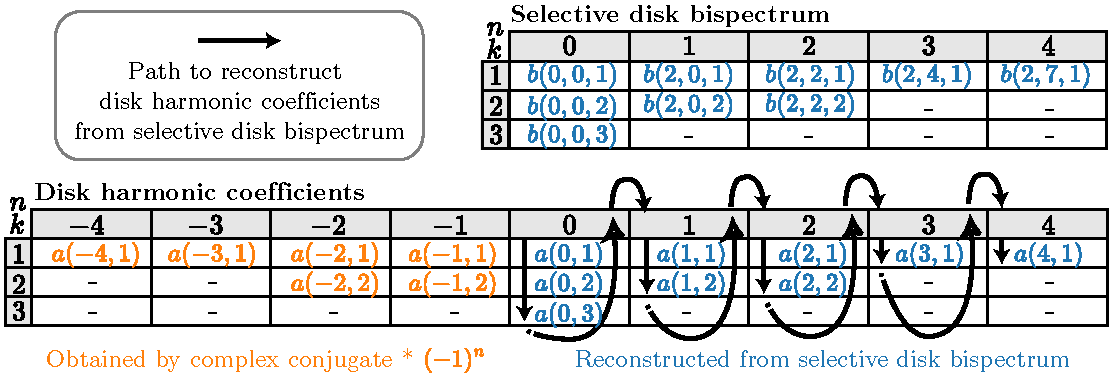
\includegraphics[width=0.9\linewidth]{figs/inversion.pdf}
  \caption{Graphical illustration of the selective disk bispectrum inversion. The arrows indicate in which order the DH coefficients are reconstructed.}
  \label{fig:bispecrum_inversion}
\end{figure}

We note that our inversion of the selective disk bispectrum also yields an inversion method for the (full) disk bispectrum. We also note that nonzero coefficient assumptions (such as $a_{n, 1} \neq 0$) are classic in bispectrum inversion literature to avoid division by zero. However, this assumption does not impact real-world application as long as there is some noise on the images.

\begin{theorem}[Complete Invariance]
Let \( f \) and \( f' \) be a pair of real-valued, square-integrable functions on the disk. Let the bispectrum be defined as in Definition~\ref{def:selective-bsp}. Assume that the DH coefficients \( a_{n,1} \) of \( f \) are non-zero for all \( n \in \{0, \dots, N_m - 1\} \). Then $b^f = b^{f'}$ if and only if \( f' = f \circ R_\phi \) for any 2D rotation \( \phi \in SO(2) \). Thus, the selective bispectrum is a complete invariant.
\end{theorem}

Part of the proof relies on the equivariance of the DH coefficients, which allow us to (re)prove the invariance of the (selective) disk bispectral coefficients used in~\citep{zhao2014rotationally}. The completeness of the SDB is proven by our inversion theorem, as the SDB contains all information about the original signal necessary for reconstruction.

\begin{figure*}[t]
  \centering
  \includegraphics[width=\textwidth]{figs/bispectrum_tractability.pdf}
  \caption{(a) The selective disk bispectrum (SDB) map is significantly faster than the full disk bispectrum map, especially for large images. (b) Bispectrum invariance error decreases with higher image resolution. (c-d) The SDB coefficient inversion sucessfully reconstructs images for resolution $28\times28$ (c) and $112\times112$ (d), and achieves a similar reconstruction error as the DH Transform \cite{fast_dhcs_2023} inversion.}
  \label{fig:tractability}
\end{figure*}


\subsection{Numerical Approximation of The Selective Disk Bispectrum and Its Inversion}

To further reduce the time complexity of the selective bispectrum, we propose leveraging a recent numerical approximation of the DH coefficients \citep{fast_dhcs_2023} which computes the disk harmonic transform in $O(L^2 \log L)$. This yields the following result:

\begin{proposition}[Complexity of the selective disk bispectrum]
    Denote $L \times L$ the size of the image, $m$ the number of DH coefficients. The time complexity of the approximate selective disk bispectrum is $O(L^2 \log L + m)$.
\end{proposition}

Next, we prove that we still have precise guarantees on the accuracy of the bispectrum coefficient approximations, the invariance property, and the reconstruction of the original image.

\begin{theorem}\label{th:accuracy}
Let \( 0 < \varepsilon \leq 1 \) be a target accuracy, and assume that \( \lambda \leq \sqrt{\pi p} \) and \( |\log \varepsilon| \leq \sqrt{p} \), where $\lambda$ is the bandlimit for the DH coefficients and \( p = L^2 \) the number of pixels in the image $f$ of size $L \times L$. Let \( b^f \) and \( \tilde{b}^f \) denote the exact and approximate selective disk bispectrum of \( f \), where \( \tilde{b}^f \) is computed using the approximate disk harmonic transform of \citet{fast_dhcs_2023}. Then,
\[
\| \tilde{b}^f - b^f \|_{\infty} \leq C\varepsilon \| f \|_{1},
\]
for a constant \( C \) depending only on a bound of \( f \) on its compact disk support.
\end{theorem}

As a corollary, we find that the bispectrum coefficients are approximately invariant with controlled guarantees.

\begin{corollary}
    Let $f, f'$ be a pair of real-valued square integrable functions on the disk such that there exists a $\phi \in SO(2)$ such that $f' = f \circ R_\phi$. Under the notations and assumptions of Theorem~\ref{th:accuracy}, we have:
    \begin{equation}
        \| \tilde b^{f} - \tilde b^{f'}\|_\infty \leq 2C \varepsilon \|f\|_1,
    \end{equation}
    for a constant \( C \) depending only on a bound of \( f \) on its compact disk support.
\end{corollary}

Linking the accuracy to $f$ is useful, as it allows us to control accuracy through number of pixels $p$. If $|f|$ and $C$ are large, but we still want to reach a given accuracy, then we can choose $p$ accordingly such that $\log(\epsilon) < \sqrt{p}$) to match the desired accuracy.

\subsection{MRA with the Selective Disk Bispectrum}

We follow \cite{bendory2018bispectrum}'s assumption that $\mathbb{E}[b_i] = b^f + \delta$, where $b_i \in \{b_1, ..., B_I\}$ is the bispectrum of one rotated noisy observation, $b^f$ is the bispectrum of the true signal $f$, and $\delta$ is a bias term introduced by noise propagation in bispectrum space. In this setting, we derive $\delta$ in the setting where $b^f$ is the disk bispectrum.

\begin{proposition}[SDB MRA Correction]
     When performing MRA using the selective disk bispectrum of noisy rotated images, the mean bispectrum must be corrected by subtracting $\delta$ before inversion to image space.
     \begin{equation}
         \delta = \sigma^2[S^\dagger_{0, k_3}  \delta_{n_{j_1},0}\delta_{n_{j_2},0} + S_{01}     \delta_{1, k_3}\delta_{n_{j_2},0}+ S_{01} \delta_{1, k_3}\delta_{n_{j_1},0}]
     \end{equation}
     \label{eq:mra-correction}

\end{proposition}
